\documentclass[letterpaper, twocolumn]{article}
\usepackage{adfundem}
\usepackage{hyperref}
\usepackage{float}
\usepackage{lipsum}
\pagenumbering{gobble}



\title{Ad Fund 'Em -- Enabling Advertising in \LaTeX \ to Aid Academic Funding in a Time of Austerity}

\author{
	K.W. van Hove \\ University of Twente\\
	k.w.vanhove@utwente.nl
}

\date{April 4, 2025}





\begin{document}
	\maketitle
	
	\begin{abstract}
		Funding in academia is increasingly at risk, requiring researchers and academics to come up with alternative funding sources. Outside of academia, advertising is a popular source of revenue for many publications such as magazines and newspapers.
		
		In this paper we show how advertising in academic publications can unlock an alternative source of revenue for academics, which, with government funding worldwide on the decline, might prove a fruitful way to keep existing research ventures alive.
		
		To that extend we create ``Ad Fund 'Em'', a \LaTeX \ package which automatically adds advertisements throughout a manuscript.
	\end{abstract}
	
	\section{Introduction}
	Funding for research has declined worldwide, with many institutions facing budget cuts and financial constraints \cite{Mallapaty_2025, HogerOnderwijsPersbureau_2024}. Despite these challenges, academia continues to pursue innovation and progress, expecting researchers to uphold high standards and produce groundbreaking work. Given this reality, alternative funding sources must be explored, such as private sector investments, industry collaborations, philanthropic contributions, and competitive grants. Universities may also develop new revenue streams through research commercialization, patent licensing, and public-private partnerships. Sustaining academic research amid financial adversity requires innovative solutions and collaboration across institutions, policymakers, and the scientific community.
	
	Advertising can be a major source of revenue, playing a crucial role in funding various industries \cite{bekh2020advertising}. Advertising is deeply embedded in modern society, as illustrated in figure~\ref{fig:bus-stop} and figure~\ref{fig:mirror}. Its presence in print media dates back many years, as seen in historical examples like figure~\ref{fig:coca-cola}. One potential avenue that -- to our knowledge -- has not yet been explored is incorporating advertisements into published academic papers and manuscripts.
	
	Academic publishing is costly, with high fees for open-access publishing and expensive journal subscriptions limiting access \cite{Solomon_2012}. Yet, peer reviewers, essential to the process, work pro bono, creating a system where researchers pay to publish or access research while review labour is unpaid. By adding advertisements to these publications, some of that cost may be recouped.
	
	\textbf{Outline} -- The structure of this paper is as follows. In section~\ref{sec:setup} we explain how we create our new revenue model, in section~\ref{sec:results} we analyse how well it works, in section~\ref{sec:discussion} we discuss the meaning of these findings, in section~\ref{sec:ethics} we outline our ethical considerations for this process. Lastly, in section~\ref{sec:conclusion} we draw our conclusions.
	
	
	\begin{figure}[]
		\begin{center}
			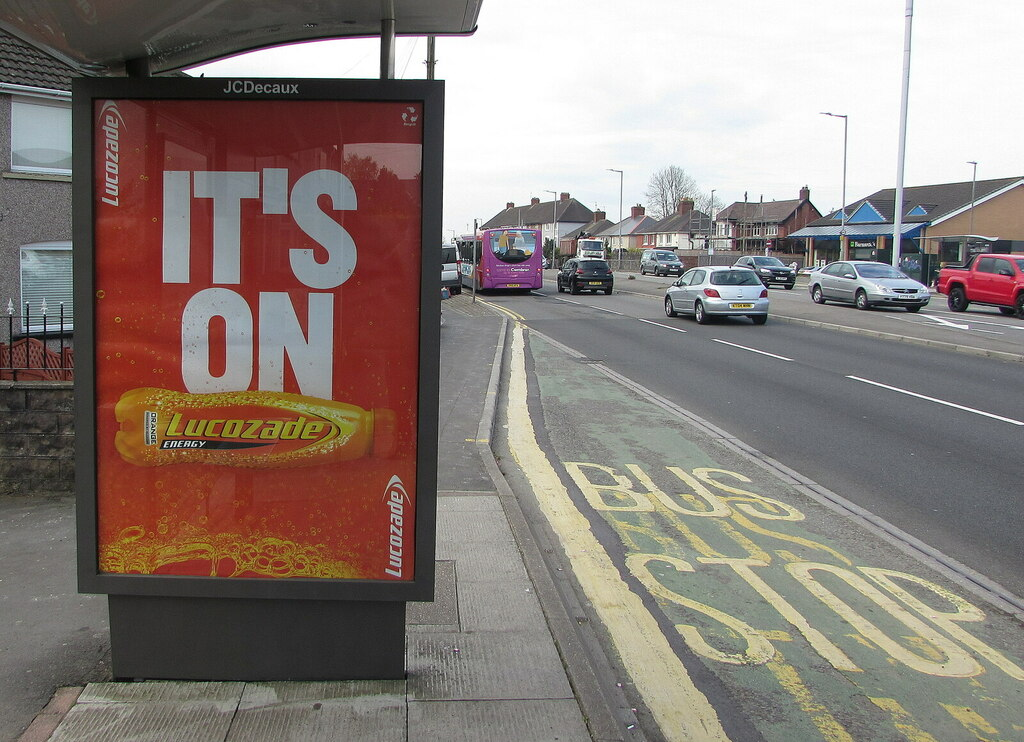
\includegraphics[width=1\linewidth]{figs/bus-stop.jpg}
			\caption{Lucozade advert on a Malpas Road bus shelter, Newport on April 27th 2021. It might be the most colourful thing in the area}
			\label{fig:bus-stop}
		\end{center}
	\end{figure}
	
	\begin{figure}[tbh]
	\begin{center}
		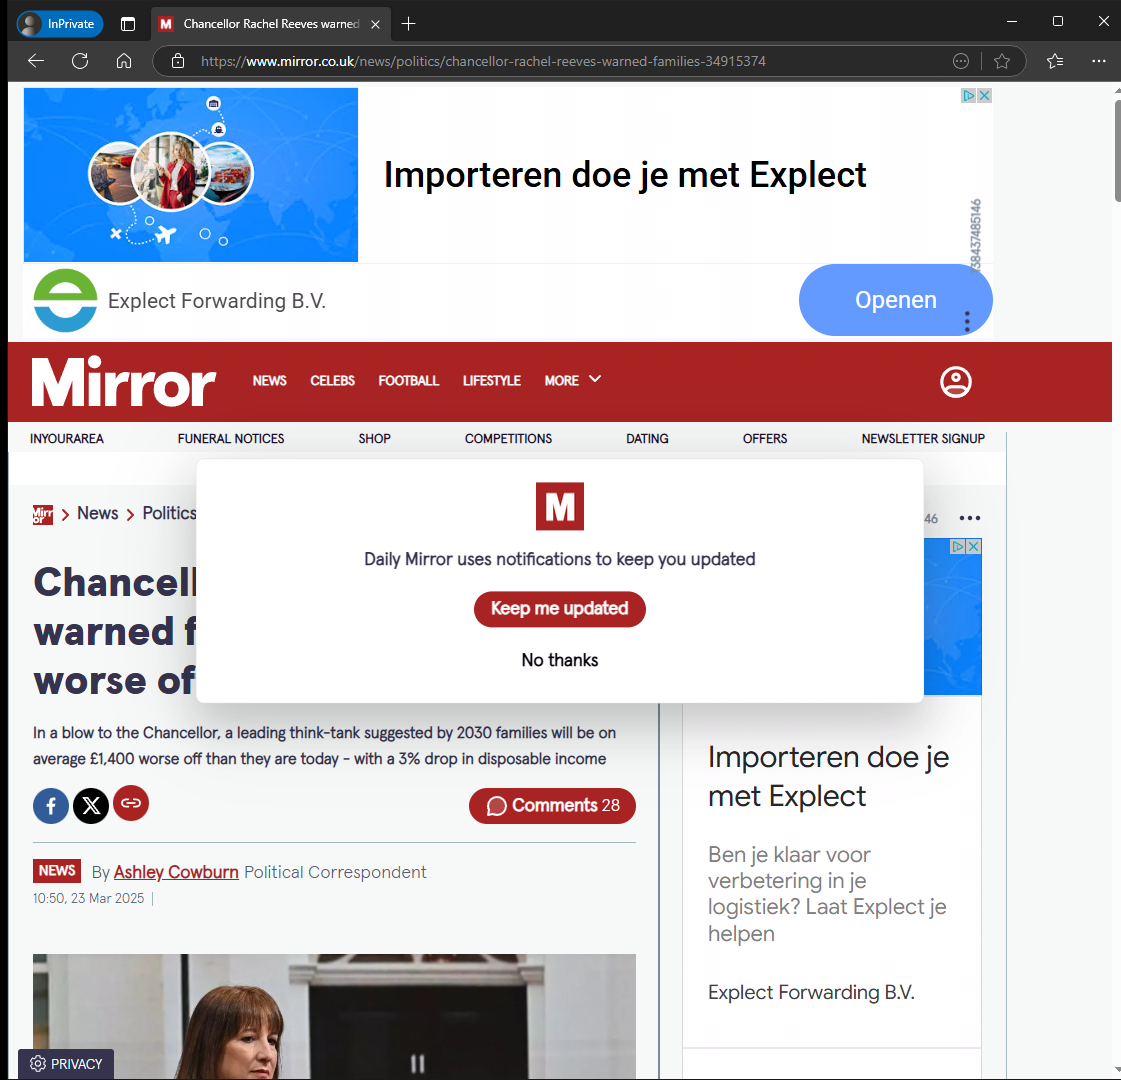
\includegraphics[width=1\linewidth]{figs/mirror.png}
		\caption{An article from the online publication The Mirror. The keen eye might spot parts of the content in between the adverts}
		\label{fig:mirror}
	\end{center}
	\end{figure} 
	
	\section{\LaTeX\ Adverts}\label{sec:setup}
	\LaTeX\ is one of the most popular languages for writing academic texts, widely used in fields such as mathematics, physics, computer science, and engineering. Unlike traditional word processors, \LaTeX\ uses a markup-based approach, allowing for greater control over formatting and document structure: \cite{Latex_2025}
	``LaTeX encourages authors not to worry too much about the appearance of their documents but to concentrate on getting the right content.''
	
	\begin{figure}[tbh]
		\begin{center}
			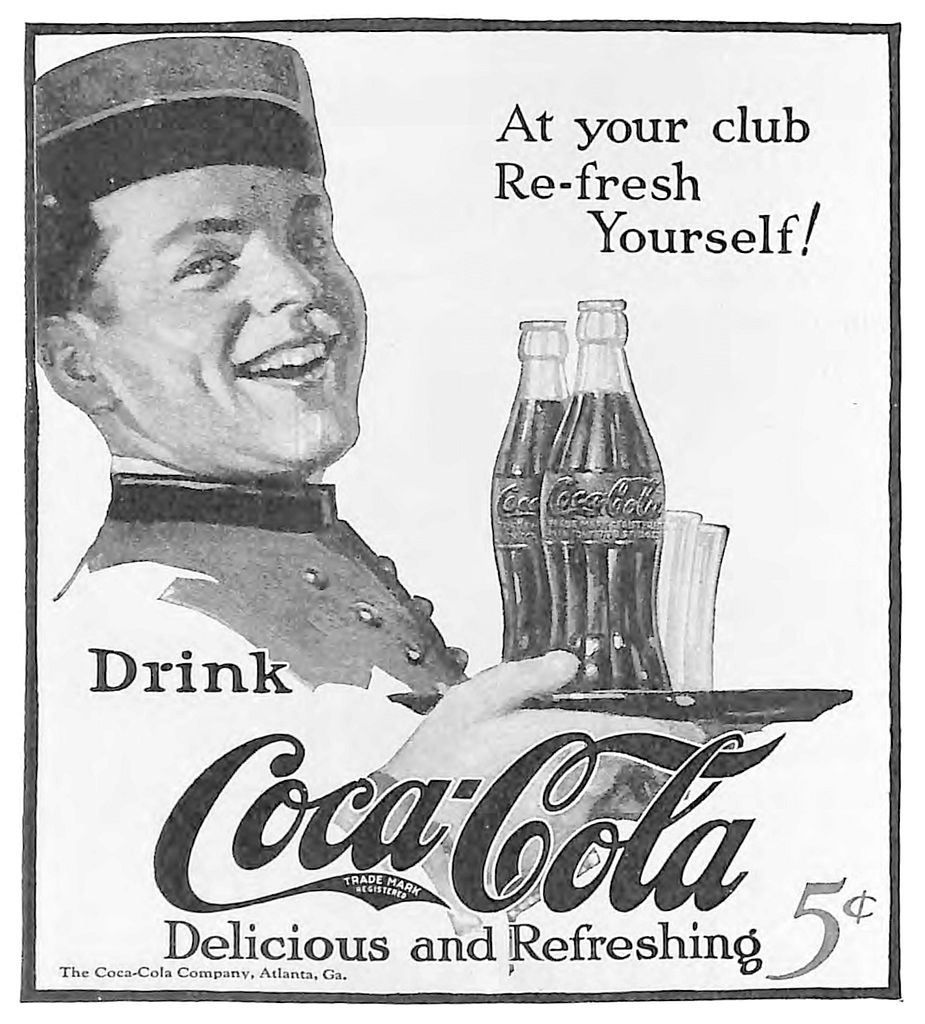
\includegraphics[width=0.9\linewidth]{figs/coca-cola.png}
			\caption{Vintage advertisement for Coca-Cola, printed in the October 1924 issue of The Elks Magazine, showing a server holding a tray with two bottles of Coca-Cola. Though even back then servers would already ask ``is Pepsi-Cola okay?'' when ordering a Coke}
			\label{fig:coca-cola}
		\end{center}
	\end{figure} 
	
	For this reason we decided to focus on \LaTeX. Our requirements were simple: we wanted it to be as simple as possible to add adverts to an already written paper. Luckily \LaTeX\ supports packages. Packages offer extra options or functionality. For that reason we decided that adding adverts should be as simple as inserting one $\verb|\usepackage{adfundem}|$ to an existing \LaTeX\ document.
	
	Because we do not want to introduce more unnecessary commands, we decided to hook in to the already existing and widely used $\verb|\section{}|$ command, which adds sections (but is also used for things like the abstract). Whenever this command is called, we prepend an advert to the document, and then execute the original command. Adverts are loaded from a folder called `ads', and are named `adN.jpg'. 
	
	\section{Results}\label{sec:results}
	You are reading one. And by reading this article you are looking at the adverts, thus potentially making us money, hence results are ever-changing.
	
	\section{Discussion}\label{sec:discussion}
	We believe this paper shows that advertising is absolutely viable. 
	
	Sadly the nature of paper (and PDFs for that matter) make dynamic adverts based on the reader not possible. This would have been a great addition. We do believe that generating the PDF dynamically with targeted adverts when the user downloads it is a viable option to increase the value of the adverts. We also would have liked to have a way to make adverts blink or play sound, but again paper does not support that.
	
	For future ventures, we also believe there might be an additional market by creating and selling an $\verb|\usepackage{adfundemadblock}|$ package which removes the ads in a published paper. 
	
	It has also been suggested to us to include a ``people who like this also like...'' section (e.g. as in figure~\ref{fig:amazon}) and call this `Related Work', but we are unsure whether that has any merit.
	
	Another suggestion that came up is more control over the nature and placement of the adverts, but we believe that the adverts themselves know best where on the page they want to be.
	
	\begin{figure}[tbh]
		\begin{center}
			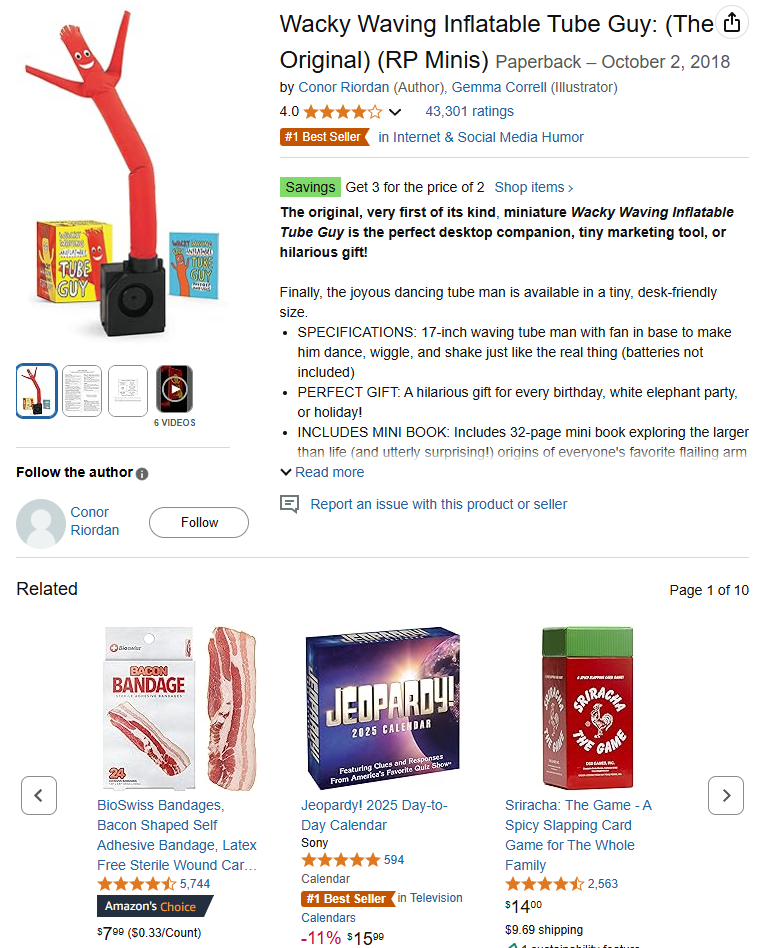
\includegraphics[width=0.9\linewidth]{figs/amazon.png}
			\caption{According to Amazon, people who like ``Wacky Waving Inflatable Tube Guy'' also like ``Bacon Shaped Self Adhesives Bandages'' -- a truly fascinating insight}
			\label{fig:amazon}
		\end{center}
	\end{figure} 

	\section{Ethical Considerations}\label{sec:ethics}
	Ethics is really important. We currently value ethics at \$10.52, but this number may change based on the revenue from our adverts.
%	
\includegraphics[width=1\linewidth]{figs/premium.png}
	
	\section{Conclusion}\label{sec:conclusion}
	Finding funding in academia is becoming increasingly difficult, with researchers and institutions facing growing financial constraints. This paper presents an alternative approach to generating revenue by incorporating advertisements into academic manuscripts. To illustrate this concept, the paper itself serves as an example of how such advertising might be implemented in practice. Initial results and reactions have been promising, suggesting that this model could be a viable supplement to traditional funding sources. Further exploration is needed to assess its long-term feasibility and impact on academic publishing.
	
	\textbf{Acknowledgements --}\label{sec:acknowledgements}
	We want to thank \href{https://www.freepik.com/author/graphicforest}{GraphicForest} for the excellent advertisement placeholders. And Jaggery for the bus stop picture.
	
	\textbf{Code --}
	All code for Ad Fund 'Em is available under a permissive licence on GitHub -- \url{https://github.com/Koenvh1/adfundem}.
	
	
	
	
	\bibliographystyle{acm} 
	\bibliography{paper}
	%inline the .bbl file directly for mailing to authors.
	
\end{document}
